\chapter{System architecture}
\label{cha:architecture}

This section describes the system architecture of our solution.


% --------------------------------------------------------------------------- %
% Components
% --------------------------------------------------------------------------- %
\section{Components}
\label{sec:components}

Our system consist of three logical parts: Java classes, input files and ouput
files. We also made use of some external libraries, which are described in
\hyperref[sec:external-libraries]{Section \ref*{sec:external-libraries}}.
\hyperref[fig:system-overview]{Figure \ref*{fig:system-overview}} shows an
overview of the system components.

\begin{figure}[htb]
\begin{center}
	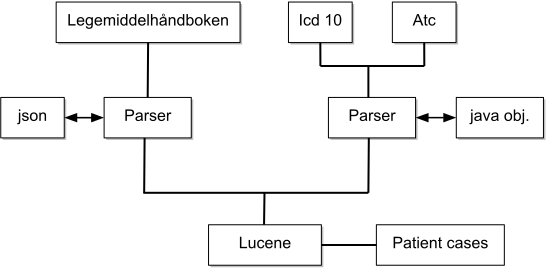
\includegraphics[width=\textwidth]{figures/system-overview}
\end{center}
\caption{System overview}
\label{fig:system-overview}
\end{figure}


% --------------------------------------------------------------------------- %
% External libraries
% --------------------------------------------------------------------------- %
\section{External libraries}
\label{sec:external-libraries}

\subsection*{Jsoup}
Jsoup is an open source Java library for working with real-world HTML. It
provides a very convenient API for extracting and manipulating data. We use
Jsoup during the parsing of Legemiddelhåndboka.\\\\
\url{http://jsoup.org/}

\subsection*{The OWL API}
The OWL API is an open source Java library used when working with OWL
ontologies. We use this API when we’re retrieving information from the ICD-10
OWL ontology.\\\\
\url{http://OWLAPI.sourceforge.net/}

\subsection*{JSON.simple}
JSON simple is a Java toolkit that are used to encode/decode JSON text. We use
this to when we want to save the chapters of Legemiddelhåndboka. We chose
JSON.simple because it provides a very simple and basic tool to convert Java
objects to JSON text, which is just what we needed.\\\\
\url{https://code.google.com/p/json-simple/}

\subsection*{Lucene}
Apache Lucene is an open source text search engine library written in Java. We
use Lucene for all our indexing/searching operation in our solution.\\\\
\url{http://Lucene.apache.org/core/}


% --------------------------------------------------------------------------- %
% Java classes
% --------------------------------------------------------------------------- %
\section{Java classes}
\label{sec:java-classes}

\begin{figure}[htb]
\begin{center}
    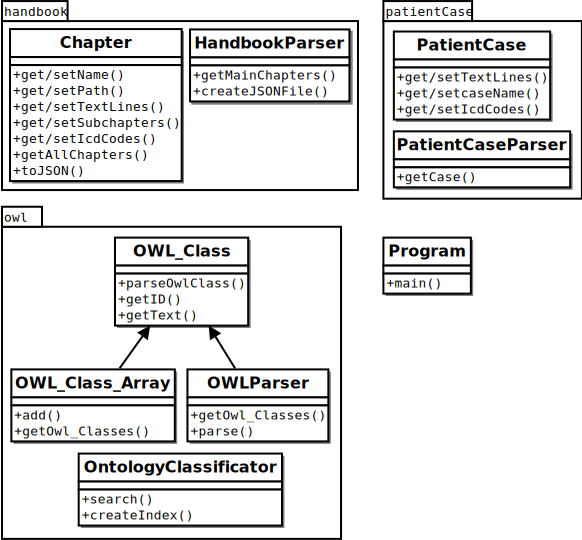
\includegraphics[width=\textwidth]{figures/class-diagram}
\end{center}
\caption{Class diagram}
\label{fig:class-diagram}
\end{figure}

% vim: set ts=2 sw=2 tw=80:
